%!TeX root=../sensetop.tex
\chapter[Chapter \thechapter]{}
\lettrine[lines=4,lraise=0.3]{W}{hen} the particulars of this conversation were repeated by Miss Dashwood to her sister, as they very soon were, the effect on her was not entirely such as the former had hoped to see. Not that Marianne appeared to distrust the truth of any part of it, for she listened to it all with the most steady and submissive attention, made neither objection nor remark, attempted no vindication of Willoughby, and seemed to show by her tears that she felt it to be impossible. But though this behaviour assured Elinor that the conviction of this guilt was carried home to her mind, though she saw with satisfaction the effect of it, in her no longer avoiding Colonel Brandon when he called, in her speaking to him, even voluntarily speaking, with a kind of compassionate respect, and though she saw her spirits less violently irritated than before, she did not see her less wretched. Her mind did become settled, but it was settled in a gloomy dejection. She felt the loss of Willoughby’s character yet more heavily than she had felt the loss of his heart; his seduction and desertion of Miss Williams, the misery of that poor girl, and the doubt of what his designs might \textit{once} have been on herself, preyed altogether so much on her spirits, that she could not bring herself to speak of what she felt even to Elinor; and, brooding over her sorrows in silence, gave more pain to her sister than could have been communicated by the most open and most frequent confession of them.

To give the feelings or the language of Mrs Dashwood on receiving and answering Elinor’s letter would be only to give a repetition of what her daughters had already felt and said; of a disappointment hardly less painful than Marianne’s, and an indignation even greater than Elinor’s. Long letters from her, quickly succeeding each other, arrived to tell all that she suffered and thought; to express her anxious solicitude for Marianne, and entreat she would bear up with fortitude under this misfortune. Bad indeed must the nature of Marianne’s affliction be, when her mother could talk of fortitude! mortifying and humiliating must be the origin of those regrets, which \textit{she} could wish her not to indulge!

Against the interest of her own individual comfort, Mrs Dashwood had determined that it would be better for Marianne to be any where, at that time, than at Barton, where every thing within her view would be bringing back the past in the strongest and most afflicting manner, by constantly placing Willoughby before her, such as she had always seen him there. She recommended it to her daughters, therefore, by all means not to shorten their visit to Mrs Jennings; the length of which, though never exactly fixed, had been expected by all to comprise at least five or six weeks. A variety of occupations, of objects, and of company, which could not be procured at Barton, would be inevitable there, and might yet, she hoped, cheat Marianne, at times, into some interest beyond herself, and even into some amusement, much as the ideas of both might now be spurned by her.

From all danger of seeing Willoughby again, her mother considered her to be at least equally safe in town as in the country, since his acquaintance must now be dropped by all who called themselves her friends. Design could never bring them in each other’s way: negligence could never leave them exposed to a surprise; and chance had less in its favour in the crowd of London than even in the retirement of Barton, where it might force him before her while paying that visit at Allenham on his marriage, which Mrs Dashwood, from foreseeing at first as a probable event, had brought herself to expect as a certain one.

She had yet another reason for wishing her children to remain where they were; a letter from her son-in-law had told her that he and his wife were to be in town before the middle of February, and she judged it right that they should sometimes see their brother.

Marianne had promised to be guided by her mother’s opinion, and she submitted to it therefore without opposition, though it proved perfectly different from what she wished and expected, though she felt it to be entirely wrong, formed on mistaken grounds, and that by requiring her longer continuance in London it deprived her of the only possible alleviation of her wretchedness, the personal sympathy of her mother, and doomed her to such society and such scenes as must prevent her ever knowing a moment’s rest.

But it was a matter of great consolation to her, that what brought evil to herself would bring good to her sister; and Elinor, on the other hand, suspecting that it would not be in her power to avoid Edward entirely, comforted herself by thinking, that though their longer stay would therefore militate against her own happiness, it would be better for Marianne than an immediate return into Devonshire.

Her carefulness in guarding her sister from ever hearing Willoughby’s name mentioned, was not thrown away. Marianne, though without knowing it herself, reaped all its advantage; for neither Mrs Jennings, nor Sir John, nor even Mrs Palmer herself, ever spoke of him before her. Elinor wished that the same forbearance could have extended towards herself, but that was impossible, and she was obliged to listen day after day to the indignation of them all.

Sir John, could not have thought it possible. »A man of whom he had always had such reason to think well! Such a good-natured fellow! He did not believe there was a bolder rider in England! It was an unaccountable business. He wished him at the devil with all his heart. He would not speak another word to him, meet him where he might, for all the world! No, not if it were to be by the side of Barton covert, and they were kept watching for two hours together. Such a scoundrel of a fellow! such a deceitful dog! It was only the last time they met that he had offered him one of Folly’s puppies! and this was the end of it!«

\begin{figure}[tbph]
\centering
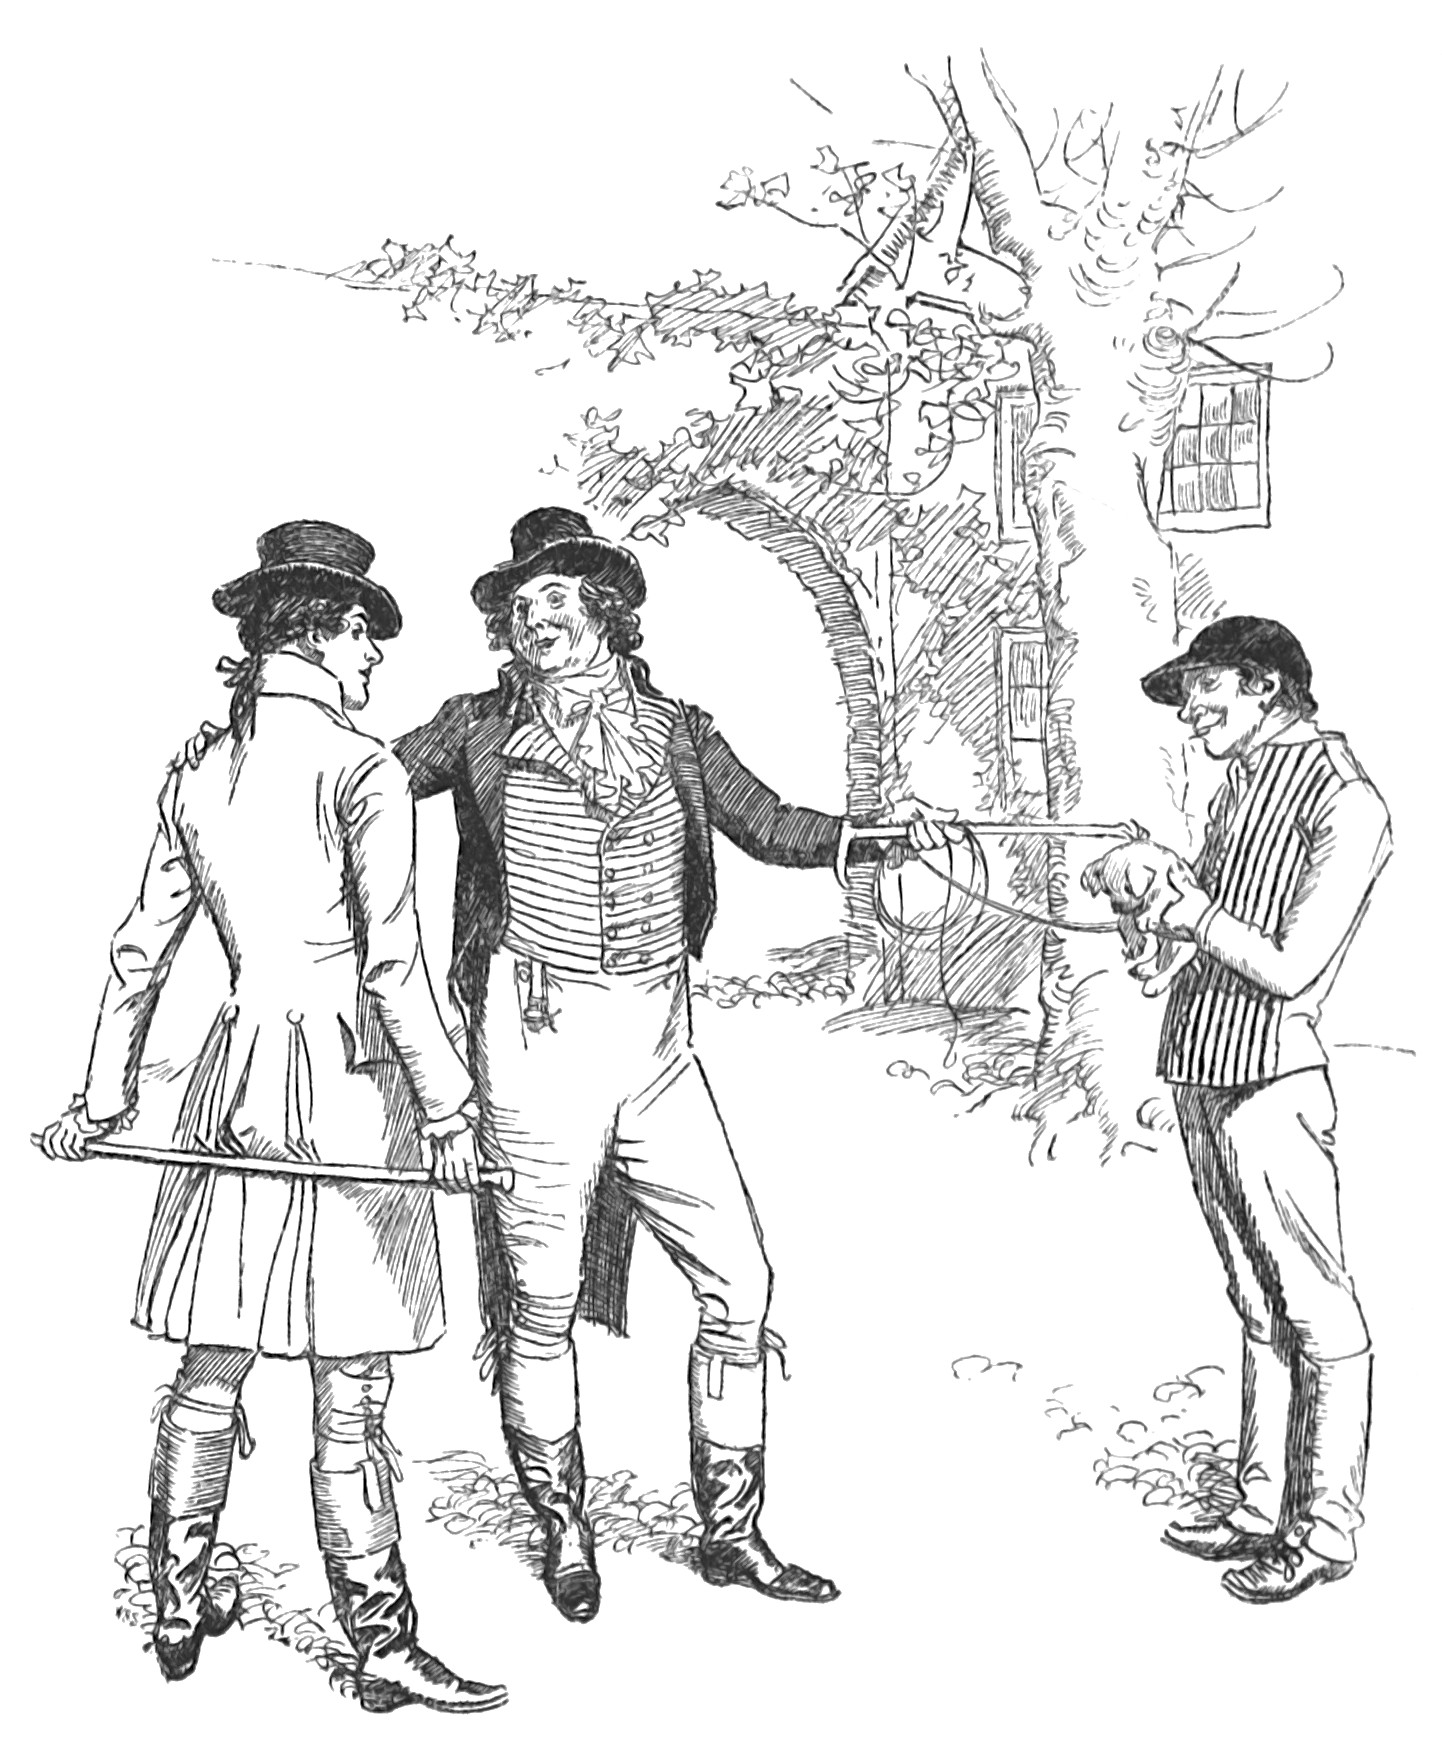
\includegraphics[width=\linewidth]{32puppies}
\caption{Offered him one of Folly’s puppies}
\end{figure}

Mrs Palmer, in her way, was equally angry. »She was determined to drop his acquaintance immediately, and she was very thankful that she had never been acquainted with him at all. She wished with all her heart Combe Magna was not so near Cleveland; but it did not signify, for it was a great deal too far off to visit; she hated him so much that she was resolved never to mention his name again, and she should tell everybody she saw, how good-for-nothing he was.«

The rest of Mrs Palmer’s sympathy was shown in procuring all the particulars in her power of the approaching marriage, and communicating them to Elinor. She could soon tell at what coachmaker’s the new carriage was building, by what painter Mr Willoughby’s portrait was drawn, and at what warehouse Miss Grey’s clothes might be seen.

The calm and polite unconcern of Lady Middleton on the occasion was a happy relief to Elinor’s spirits, oppressed as they often were by the clamorous kindness of the others. It was a great comfort to her to be sure of exciting no interest in \textit{one} person at least among their circle of friends: a great comfort to know that there was \textit{one} who would meet her without feeling any curiosity after particulars, or any anxiety for her sister’s health.

Every qualification is raised at times, by the circumstances of the moment, to more than its real value; and she was sometimes worried down by officious condolence to rate good-breeding as more indispensable to comfort than good-nature.

Lady Middleton expressed her sense of the affair about once every day, or twice, if the subject occurred very often, by saying, »It is very shocking, indeed!« and by the means of this continual though gentle vent, was able not only to see the Miss Dashwoods from the first without the smallest emotion, but very soon to see them without recollecting a word of the matter; and having thus supported the dignity of her own sex, and spoken her decided censure of what was wrong in the other, she thought herself at liberty to attend to the interest of her own assemblies, and therefore determined (though rather against the opinion of Sir John) that as Mrs Willoughby would at once be a woman of elegance and fortune, to leave her card with her as soon as she married.

Colonel Brandon’s delicate, unobtrusive enquiries were never unwelcome to Miss Dashwood. He had abundantly earned the privilege of intimate discussion of her sister’s disappointment, by the friendly zeal with which he had endeavoured to soften it, and they always conversed with confidence. His chief reward for the painful exertion of disclosing past sorrows and present humiliations, was given in the pitying eye with which Marianne sometimes observed him, and the gentleness of her voice whenever (though it did not often happen) she was obliged, or could oblige herself to speak to him. \textit{These} assured him that his exertion had produced an increase of good-will towards himself, and \textit{these} gave Elinor hopes of its being farther augmented hereafter; but Mrs Jennings, who knew nothing of all this, who knew only that the Colonel continued as grave as ever, and that she could neither prevail on him to make the offer himself, nor commission her to make it for him, began, at the end of two days, to think that, instead of Midsummer, they would not be married till Michaelmas, and by the end of a week that it would not be a match at all. The good understanding between the Colonel and Miss Dashwood seemed rather to declare that the honours of the mulberry-tree, the canal, and the yew arbour, would all be made over to \textit{her}; and Mrs Jennings had, for some time ceased to think at all of Mrs Ferrars.

Early in February, within a fortnight from the receipt of Willoughby’s letter, Elinor had the painful office of informing her sister that he was married. She had taken care to have the intelligence conveyed to herself, as soon as it was known that the ceremony was over, as she was desirous that Marianne should not receive the first notice of it from the public papers, which she saw her eagerly examining every morning.

She received the news with resolute composure; made no observation on it, and at first shed no tears; but after a short time they would burst out, and for the rest of the day, she was in a state hardly less pitiable than when she first learnt to expect the event.

The Willoughbys left town as soon as they were married; and Elinor now hoped, as there could be no danger of her seeing either of them, to prevail on her sister, who had never yet left the house since the blow first fell, to go out again by degrees as she had done before.

About this time the two Miss Steeles, lately arrived at their cousin’s house in Bartlett’s Buildings, Holburn, presented themselves again before their more grand relations in Conduit and Berkeley Streets; and were welcomed by them all with great cordiality.

Elinor only was sorry to see them. Their presence always gave her pain, and she hardly knew how to make a very gracious return to the overpowering delight of Lucy in finding her \textit{still} in town.

»I should have been quite disappointed if I had not found you here \textit{still},« said she repeatedly, with a strong emphasis on the word. »But I always thought I \textit{should}. I was almost sure you would not leave London yet awhile; though you \textit{told} me, you know, at Barton, that you should not stay above a \textit{month}. But I thought, at the time, that you would most likely change your mind when it came to the point. It would have been such a great pity to have went away before your brother and sister came. And now to be sure you will be in no \textit{hurry} to be gone. I am amazingly glad you did not keep to \textit{your word}.«

Elinor perfectly understood her, and was forced to use all her self-command to make it appear that she did \textit{not}.

»Well, my dear,« said Mrs Jennings, »and how did you travel?«

»Not in the stage, I assure you,« replied Miss Steele, with quick exultation; »we came post all the way, and had a very smart beau to attend us. Dr Davies was coming to town, and so we thought we’d join him in a post-chaise; and he behaved very genteelly, and paid ten or twelve shillings more than we did.«

\begin{figure}[tbph]
\centering

\includegraphics[width=\linewidth]{32beau}
\caption{A very smart beau}
\end{figure}

»Oh, oh!« cried Mrs Jennings; »very pretty, indeed! and the Doctor is a single man, I warrant you.«

»There now,« said Miss Steele, affectedly simpering, »everybody laughs at me so about the Doctor, and I cannot think why. My cousins say they are sure I have made a conquest; but for my part I declare I never think about him from one hour’s end to another. »Lord! here comes your beau, Nancy,« my cousin said t’other day, when she saw him crossing the street to the house. My beau, indeed! said I—I cannot think who you mean. The Doctor is no beau of mine.«

»Aye, aye, that is very pretty talking—but it won’t do—the Doctor is the man, I see.«

»No, indeed!« replied her cousin, with affected earnestness, »and I beg you will contradict it, if you ever hear it talked of.«

Mrs Jennings directly gave her the gratifying assurance that she certainly would \textit{not}, and Miss Steele was made completely happy.

»I suppose you will go and stay with your brother and sister, Miss Dashwood, when they come to town,« said Lucy, returning, after a cessation of hostile hints, to the charge.

»No, I do not think we shall.«

»Oh, yes, I dare say you will.«

Elinor would not humour her by farther opposition.

»What a charming thing it is that Mrs Dashwood can spare you both for so long a time together!«

»Long a time, indeed!« interposed Mrs Jennings. »Why, their visit is but just begun!«

Lucy was silenced.

»I am sorry we cannot see your sister, Miss Dashwood,« said Miss Steele. »I am sorry she is not well\longdash« for Marianne had left the room on their arrival.

»You are very good. My sister will be equally sorry to miss the pleasure of seeing you; but she has been very much plagued lately with nervous head-aches, which make her unfit for company or conversation.«

»Oh, dear, that is a great pity! but such old friends as Lucy and me!—I think she might see \textit{us}; and I am sure we would not speak a word.«

Elinor, with great civility, declined the proposal. Her sister was perhaps laid down upon the bed, or in her dressing gown, and therefore not able to come to them.

»Oh, if that’s all,« cried Miss Steele, »we can just as well go and see \textit{her}.«

Elinor began to find this impertinence too much for her temper; but she was saved the trouble of checking it, by Lucy’s sharp reprimand, which now, as on many occasions, though it did not give much sweetness to the manners of one sister, was of advantage in governing those of the other.